\documentclass[fleqn,12pt]{project}

\setlength{\columnsep}{0.55cm}
\setlength{\fboxrule}{0.75pt}

\definecolor{color1}{RGB}{0,0,90}
\definecolor{color2}{RGB}{0,20,20}

\usepackage{multirow}
\usepackage{tcolorbox,listings}
\lstset{
	showstringspaces=false,
  tabsize=2,
  breaklines=true,
  columns=fullflexible
}
\tcbuselibrary{breakable}

\usepackage{hyperref}
\hypersetup{hidelinks,colorlinks,breaklinks=true,urlcolor=color2,citecolor=color1,linkcolor=color1,bookmarksopen=false,pdftitle={Title},pdfauthor={Author}}

\JournalInfo{

\includegraphics[width=2.5cm]{Figures/engineering-logo}
\Archive{}
}

\PaperTitle{ENR 280 Design Project Report (Fall 2022)}
\Authors{\textbf{Green Team:} Kristine Kalthoff, Isaac Anderson, Jonathan Ganzer, Austin Barchenger\textsuperscript{1}*.}
\affiliation{\textsuperscript{1}\textit{School of Engineering, 
  University of Mary, Bismarck, North Dakota}}
\affiliation{*ajgarcia@umary.edu}


\Keywords{}
\newcommand{\keywordname}{Keywords}

\Abstract{
   This design report documents the background, theory, ideas, methodology of the design process, designs, proposed manufacturing techniques, prototypes, management, and analysis for the remote control car, dynamic elevator, and static bridge our group will design and prototype. The objective of this design project is to practically apply the material learned in technical engineering courses and to experience the process of designing and managing an engineering project.   
\
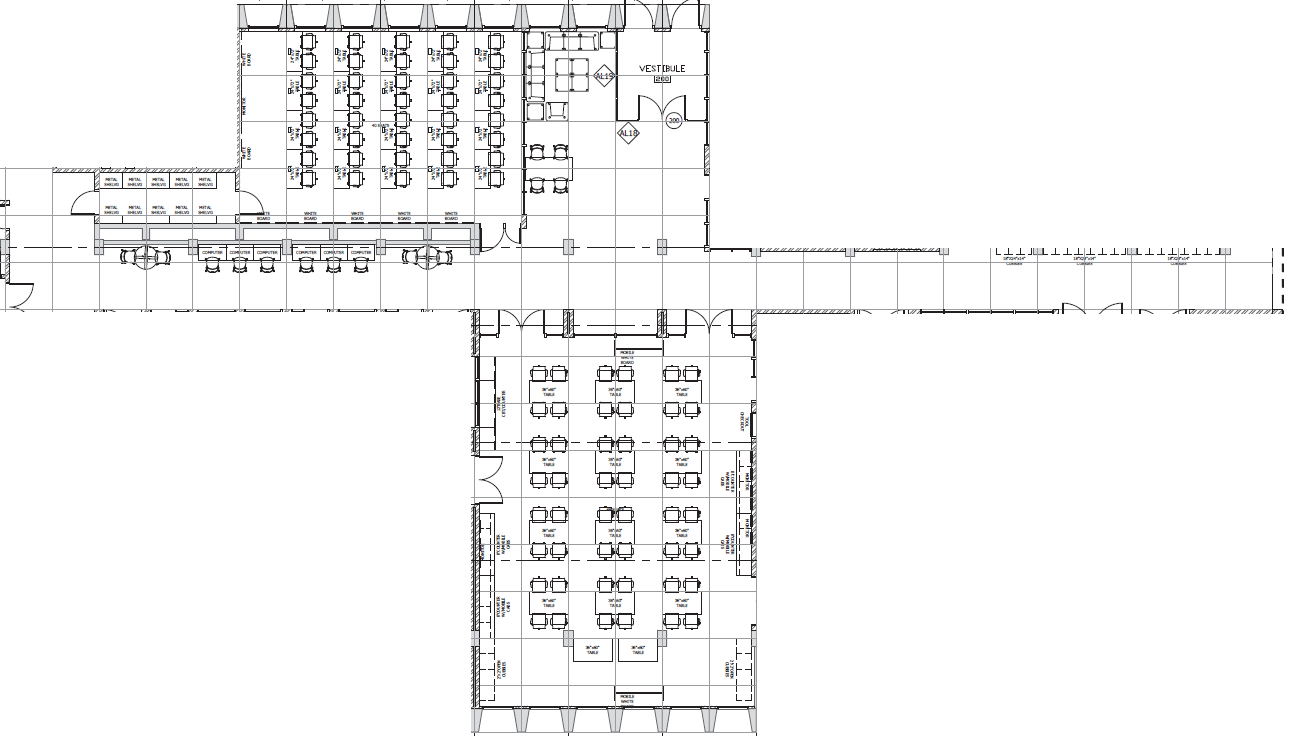
\includegraphics[width=17cm]{Figures/Floorplan}
}

\begin{document}

\flushbottom
\maketitle
\newpage
\tableofcontents
\thispagestyle{empty}
\newpage
\section*{Executive Summary}
\addcontentsline{toc}{section}{Executive Summary}

\newpage
\section{Design Problem and Objectives}

 The project assigned to each group is to design a remote control car and parts of the race track, which includes designing both a dynamic and static structure. Our group in particular was assigned an elevator as our dynamic structure and a bridge as our static structure. The race course will be constructed in the University of Mary Engineering Building and occupy the Senior Design Center, Engineering Fundamentals classroom, and the Engineering building hallway and lobby depicted in Figure \ref{fig:Fig1}. In this course, ENR 280 students are tasked to present and document designs and prototypes that would be ready for manufacturing, which will take place in the sequent class, ENR 281 - Engineering Design Lab 2. Course deliverables include a detailed project report, prototypes of designs, and a presentation. 

\begin{figure}\centering
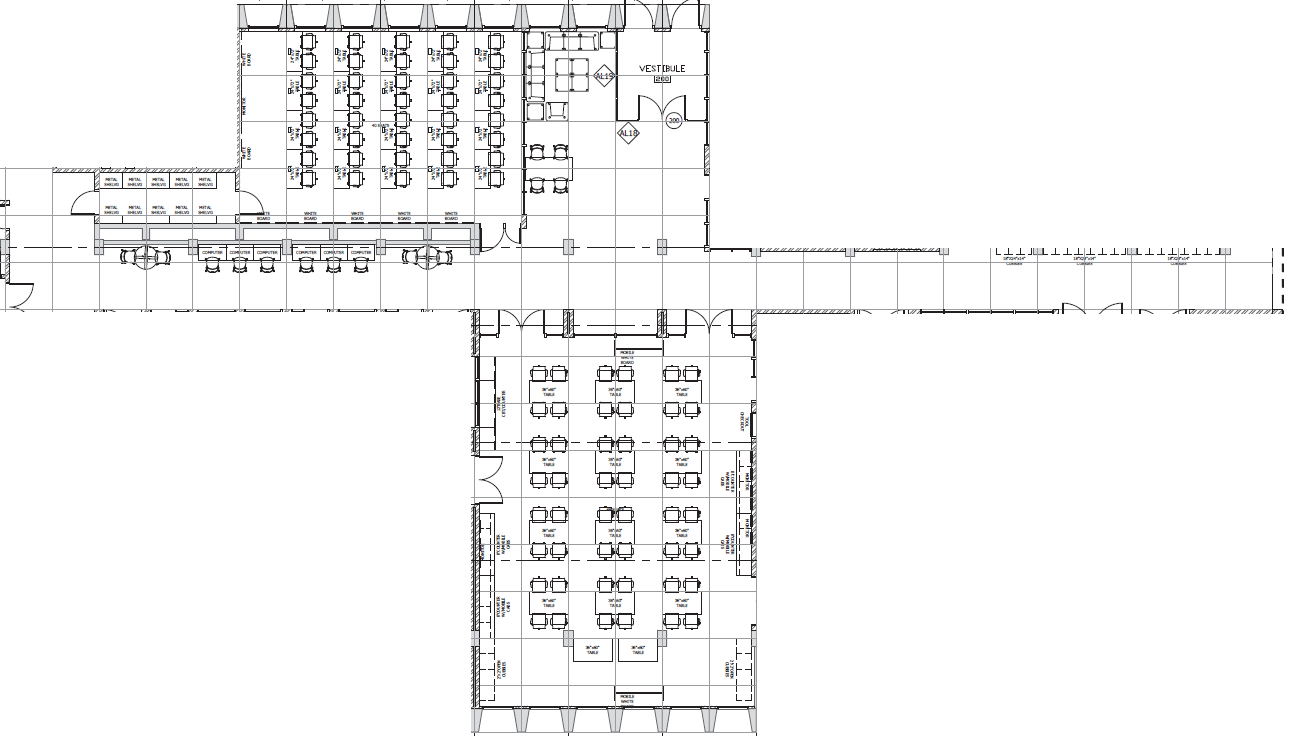
\includegraphics[width=17cm]{Figures/Floorplan}
\caption{Engineering Building Space for the Marauder's Cart course}
\label{fig:Fig1}
\end{figure}
\subsection{Design Specifications}

Each of these designs had to satisfy the requirements set out by the professor and our assigned client. A breakdown of the specifications required of our team's design items are stated in Table \ref{table:Table1}. In addition to these specifications, an overall budget of \$450 was given to meet these needs.  

\begin{table}
\caption{Design Specifications}
\begin{center}
\small
\begin{tabular}{|cl|}
\hline
\bf{Need}\phantom{11000000000}&
\begin{tabular}{|p{5.5cm}|p{7cm}}
\bf{Design} & \bf{Specifications} \\
\end{tabular}\\
\hline
\end{tabular}
\begin{tabular}{|cl|}
\hline
Car \phantom{110000000000} &
\begin{tabular}{|p{5.5cm}|p{7cm}}
Arduino remote controlled car & Max Dimensions: 12"x 8"x 8", 7 lbs  \\
 & No weapons/hacking/signal jamming    \\
  & 4 separately driven wheels with great traction    \\
   &  Braking System   \\
    & Batman themed    \\
 \end{tabular}\\
\hline
\end{tabular}
\begin{tabular}{|cl|}
\hline
Dynamic Structure &
\begin{tabular}{|p{5.5cm}|p{7cm}}
 Elevator & Transport cars from tabletop down to floor    \\
  & Max Cargo Load: 7lbs    \\
  & Traverse Distance (height of table): TBD    \\
  & Design must involve water  \\
 \end{tabular}\\
\hline
\end{tabular}
\begin{tabular}{|cl|}
\hline
Static Structure \phantom{N0}&
\begin{tabular}{|p{5.5cm}|p{7cm}}
 Bridge  & Span: TBD \\
   & Involve ice or slippery surface that mimics ice    \\
 \end{tabular}\\
\hline
\end{tabular}
\end{center}
\label{table:Table1}
\end{table}


\subsection{Project Objectives}
The purpose and prime objective of the design project is for us to experience the entire design process and create a document that outlines the background, theory, ideas, methodology of the design process,
designs, proposed manufacturing techniques, prototypes, management, and analysis for the remote control car and various structures
students will design and prototype. The objective of this design project is to practically apply the material students learn in their
technical engineering courses and from their own independent research, and to experience the process of designing and managing an engineering project.

%%%%%%%%%%%%%%%%%%%%%%%%%%%%%%%%%%%%%%%%%%%%%%%%%%%%%%%%%%%%%%%%%%%%%%%%%%%%%%%%%%%%%%%%%%%%%%%%%%%%
\newpage
\section{Literature Review}

Introduce the areas that will be covered in the literature review and why. Focus on the theory and background of the topics you are discussing, present what the a reader looking to duplicate your work would really need to know before trying to understand your design work.

\subsection{Elevators}
For example, in order to be able to design a Jump Ramp one has to have a good understanding of how to calculate projectiles. So you'll want to present a basic explanation of the concept of what a jump ramp is and \textbf{relevant equations so the reader now has enough understanding to interpret your design work.} 
So for a understanding a projectile, one needs to know that the only acceleration that the body experiences during it's flight is gravity. This allows us to use simplified kinematic equations in a two dimensional space as all accelerations are known and are constants. Equations \ref{eq:y} and \ref{eq:x} below are  kinematic equations that describe the position of a projectile in the x and y directions with respect to time.

\begin{equation}
	y = y_0 + (v_0)_yt + \frac{1}{2}a_yt^2
\label{eq:y}
\end{equation}
\begin{equation}
	x = x_0 + (x_0)_xt
\label{eq:x}
\end{equation}
\begin{itemize}
\item x or y is final position in it's respective direction.
\item $x_0$ or $y_0$ is the initial position in it's respective direction.
\item $(v_0)_x$ or $(v_0)_y$ is the initial velocity in it's respective direction.
\item $a_y$ is the Acceleration in the y direction (this is gravity, the only acceleration the projectile experiences).
\end{itemize}


In addition to these equations, equations derived from energy and momentum principles provide us ways to solve the projectiles without the variable of time or position, respectively. These are shown etc...

Elevators transport cargo up and down by raising and lowering their potential energy. There are numerous different ways to accomplish this, but overall elevators come in two main types: hydraulic and traction [2].

\subsubsection{Traction Elevators}
A traction elevator uses a motor at the top of the elevator shaft to turn a sheave, essentially a pulley, that is attached by cables to a counterweight and cab that carries the cargo. The counterweight is what brings efficiency to the system, without it the motor would have to do all of the work. A counterweight may weigh up to as much as the cab and 45\% of its full load, however, in this situation an empty cab would rise too quickly and resistors would need to be added to the system. Therefore, selecting a counterweight based on the desired speed and efficiency of the system is important. Faster traction elevators are gearless and the sheave is directly coupled [1]. Overall, traction elevators travel much faster than hydraulic elevators [2].

\subsubsection{Hydraulic Elevators}
Hydraulic elevators use the mechanics of a hydraulic system to raise and lower an elevator. A hydraulic system consists of a pair of connected cylinders that are filled with a fluid. Attached to the sides of the cylinders are pistons that remain in contact with the fluid. When a force is applied to one piston, the pressure is transmitted throughout the fluid and according to Pascal’s law (see Fig. 2) the pressure will be identical to that exerted in the other piston. In an elevator, the elevator cab is pushed up when a motor pushes fluid down a piston, and when the car needs to come down, a valve releases fluid from the piston [2]. Hydraulic elevators are mechanically simpler than traction elevators. 

\begin{figure}[h!]\centering
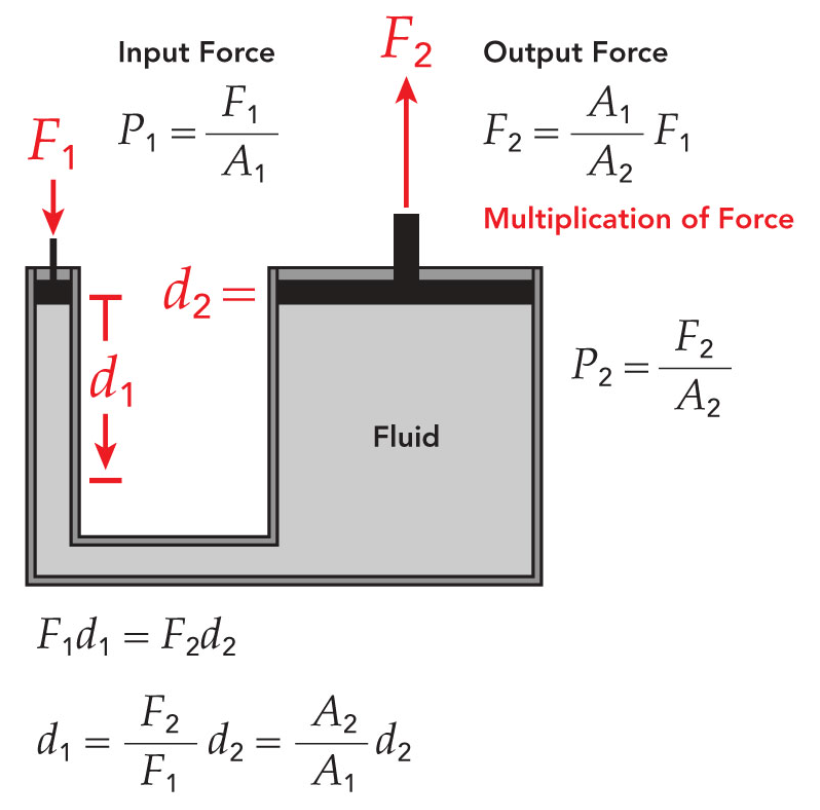
\includegraphics[width=7cm]{Pascals_Law.png}
\caption{Pascal's Law in a hydraulic lift [3]}
\label{fig:Fig1}
\end{figure}

\subsection{Bridges}

Do the same thing for bridges (or your static sturcture) here. Discuss the general information on bridges \textbf{as well as relevant theory/equations} in order to comprehend your design work. For example, in order to be able to design the bridge to satisfy the design specifications set out, one must have a basic understanding of what deflection is and how to calculate it. Here you'll want to present a basic theoretical description of what deflection is and an equation on how it can be determined. For example, for a point load, equation \ref{eq:delta}  can be used to determine the deflection at the point where the point load is applied on a beam. 

\begin{equation}
	\delta = \frac{Pa^2(L-a)^2}{3EIL} \\
\label{eq:delta}
\end{equation}

\begin{itemize}
\item $\delta$ is deflection
\item P is the point load
\item E is modulus of Elasticity
\item I is area moment of inertia
\item L is span length
\item a is the a dimension in the Point Load image shown in Figure \ref{fig:Fig2}.
\end{itemize}

Equations like this are derived and readily available for standard load cases such as point loads and distributed loads acting on a beam, as shown in Figure \ref{fig:Fig2}.
\begin{figure}\centering
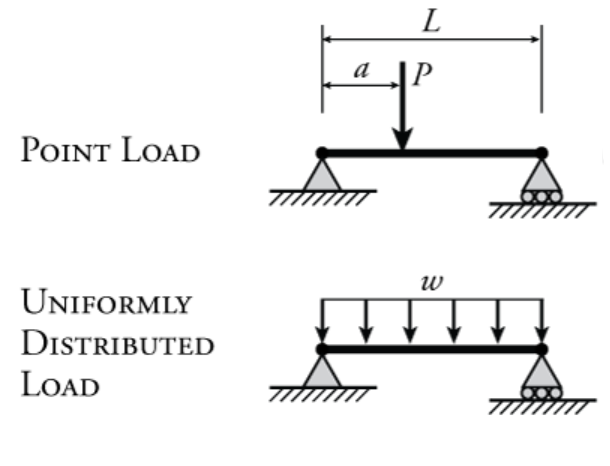
\includegraphics[width=6cm]{Figures/Loads}
\caption{Point and Distributed Loads on a Beam \cite{bib:Mechanics}}
\label{fig:Fig2}
\end{figure}

\subsection{Cars}

Discuss relevent background and theory on car frames, chassis, wheels \textbf{steering}, etc...

\subsection{Arduino Controls}
Discuss the required control logic for both the remote control car and dynamic structure. Explain any significant calculations or algorithms performed. Present the final codes with commentary as shown below.

\begin{tcolorbox}[breakable, title=\textbf{fade.h}]
\lstinputlisting[language=C++, basicstyle=\scriptsize]{Code/fade.h}
\end{tcolorbox}

Code above from \cite{bib:Fade}

%%%%%%%%%%%%%%%%%%%%%%%%%%%%%%%%%%%%%%%%%%%%%%%%%%%%%%%%%%%%%%%%%%%%%%%%%%%%%%%%%%%%%%%%%%%%%%%%%%%%
\newpage
\section{Design Conceptualization, Initial Ideas, Process and Decisions}

\subsection{Design Concepts and Initial Ideas}
\subsubsection{Elevator}

\begin{figure}[h!]\centering
\begin{subfigure}
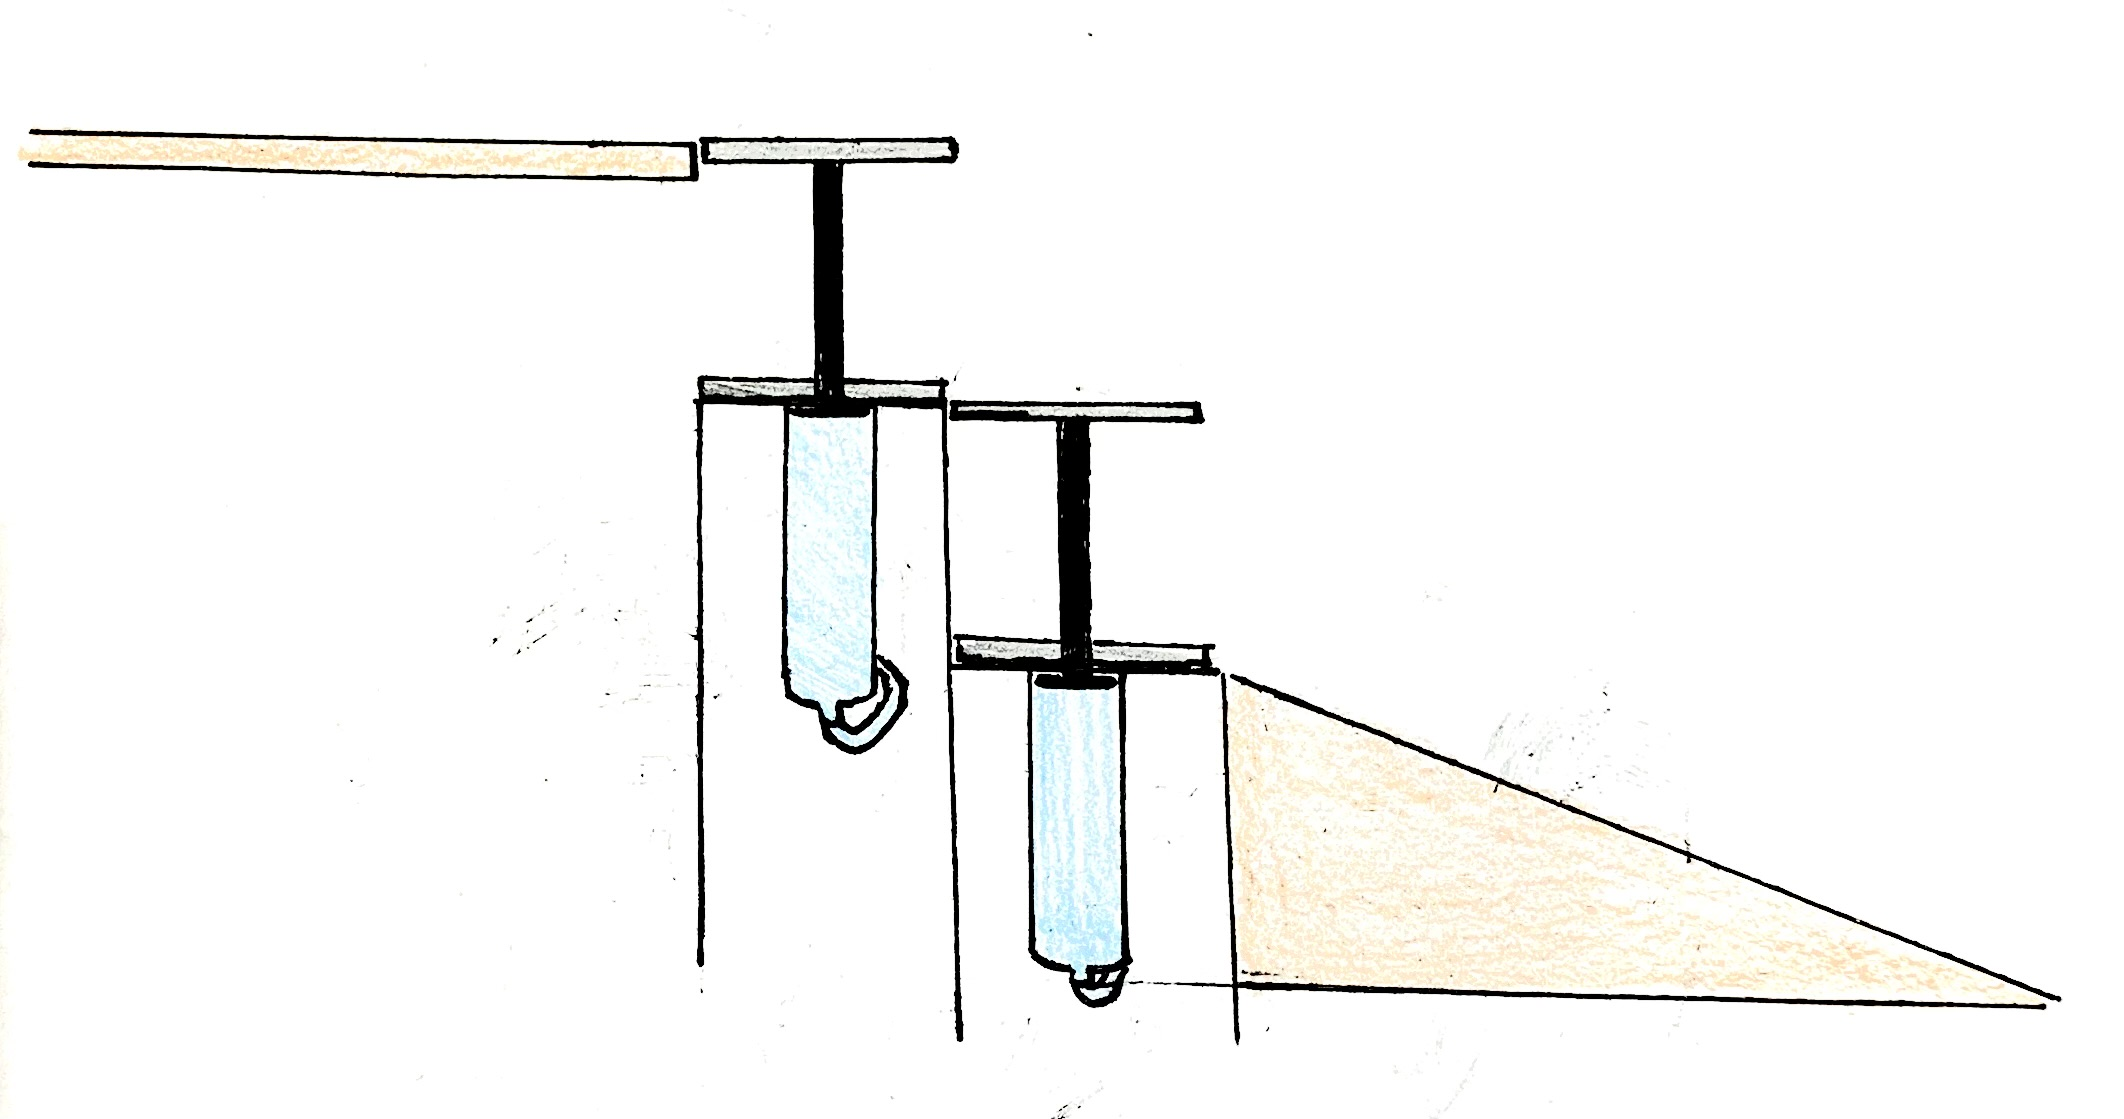
\includegraphics[width=9cm]{IMG_8471.jpg}
\end{subfigure}
\begin{subfigure}
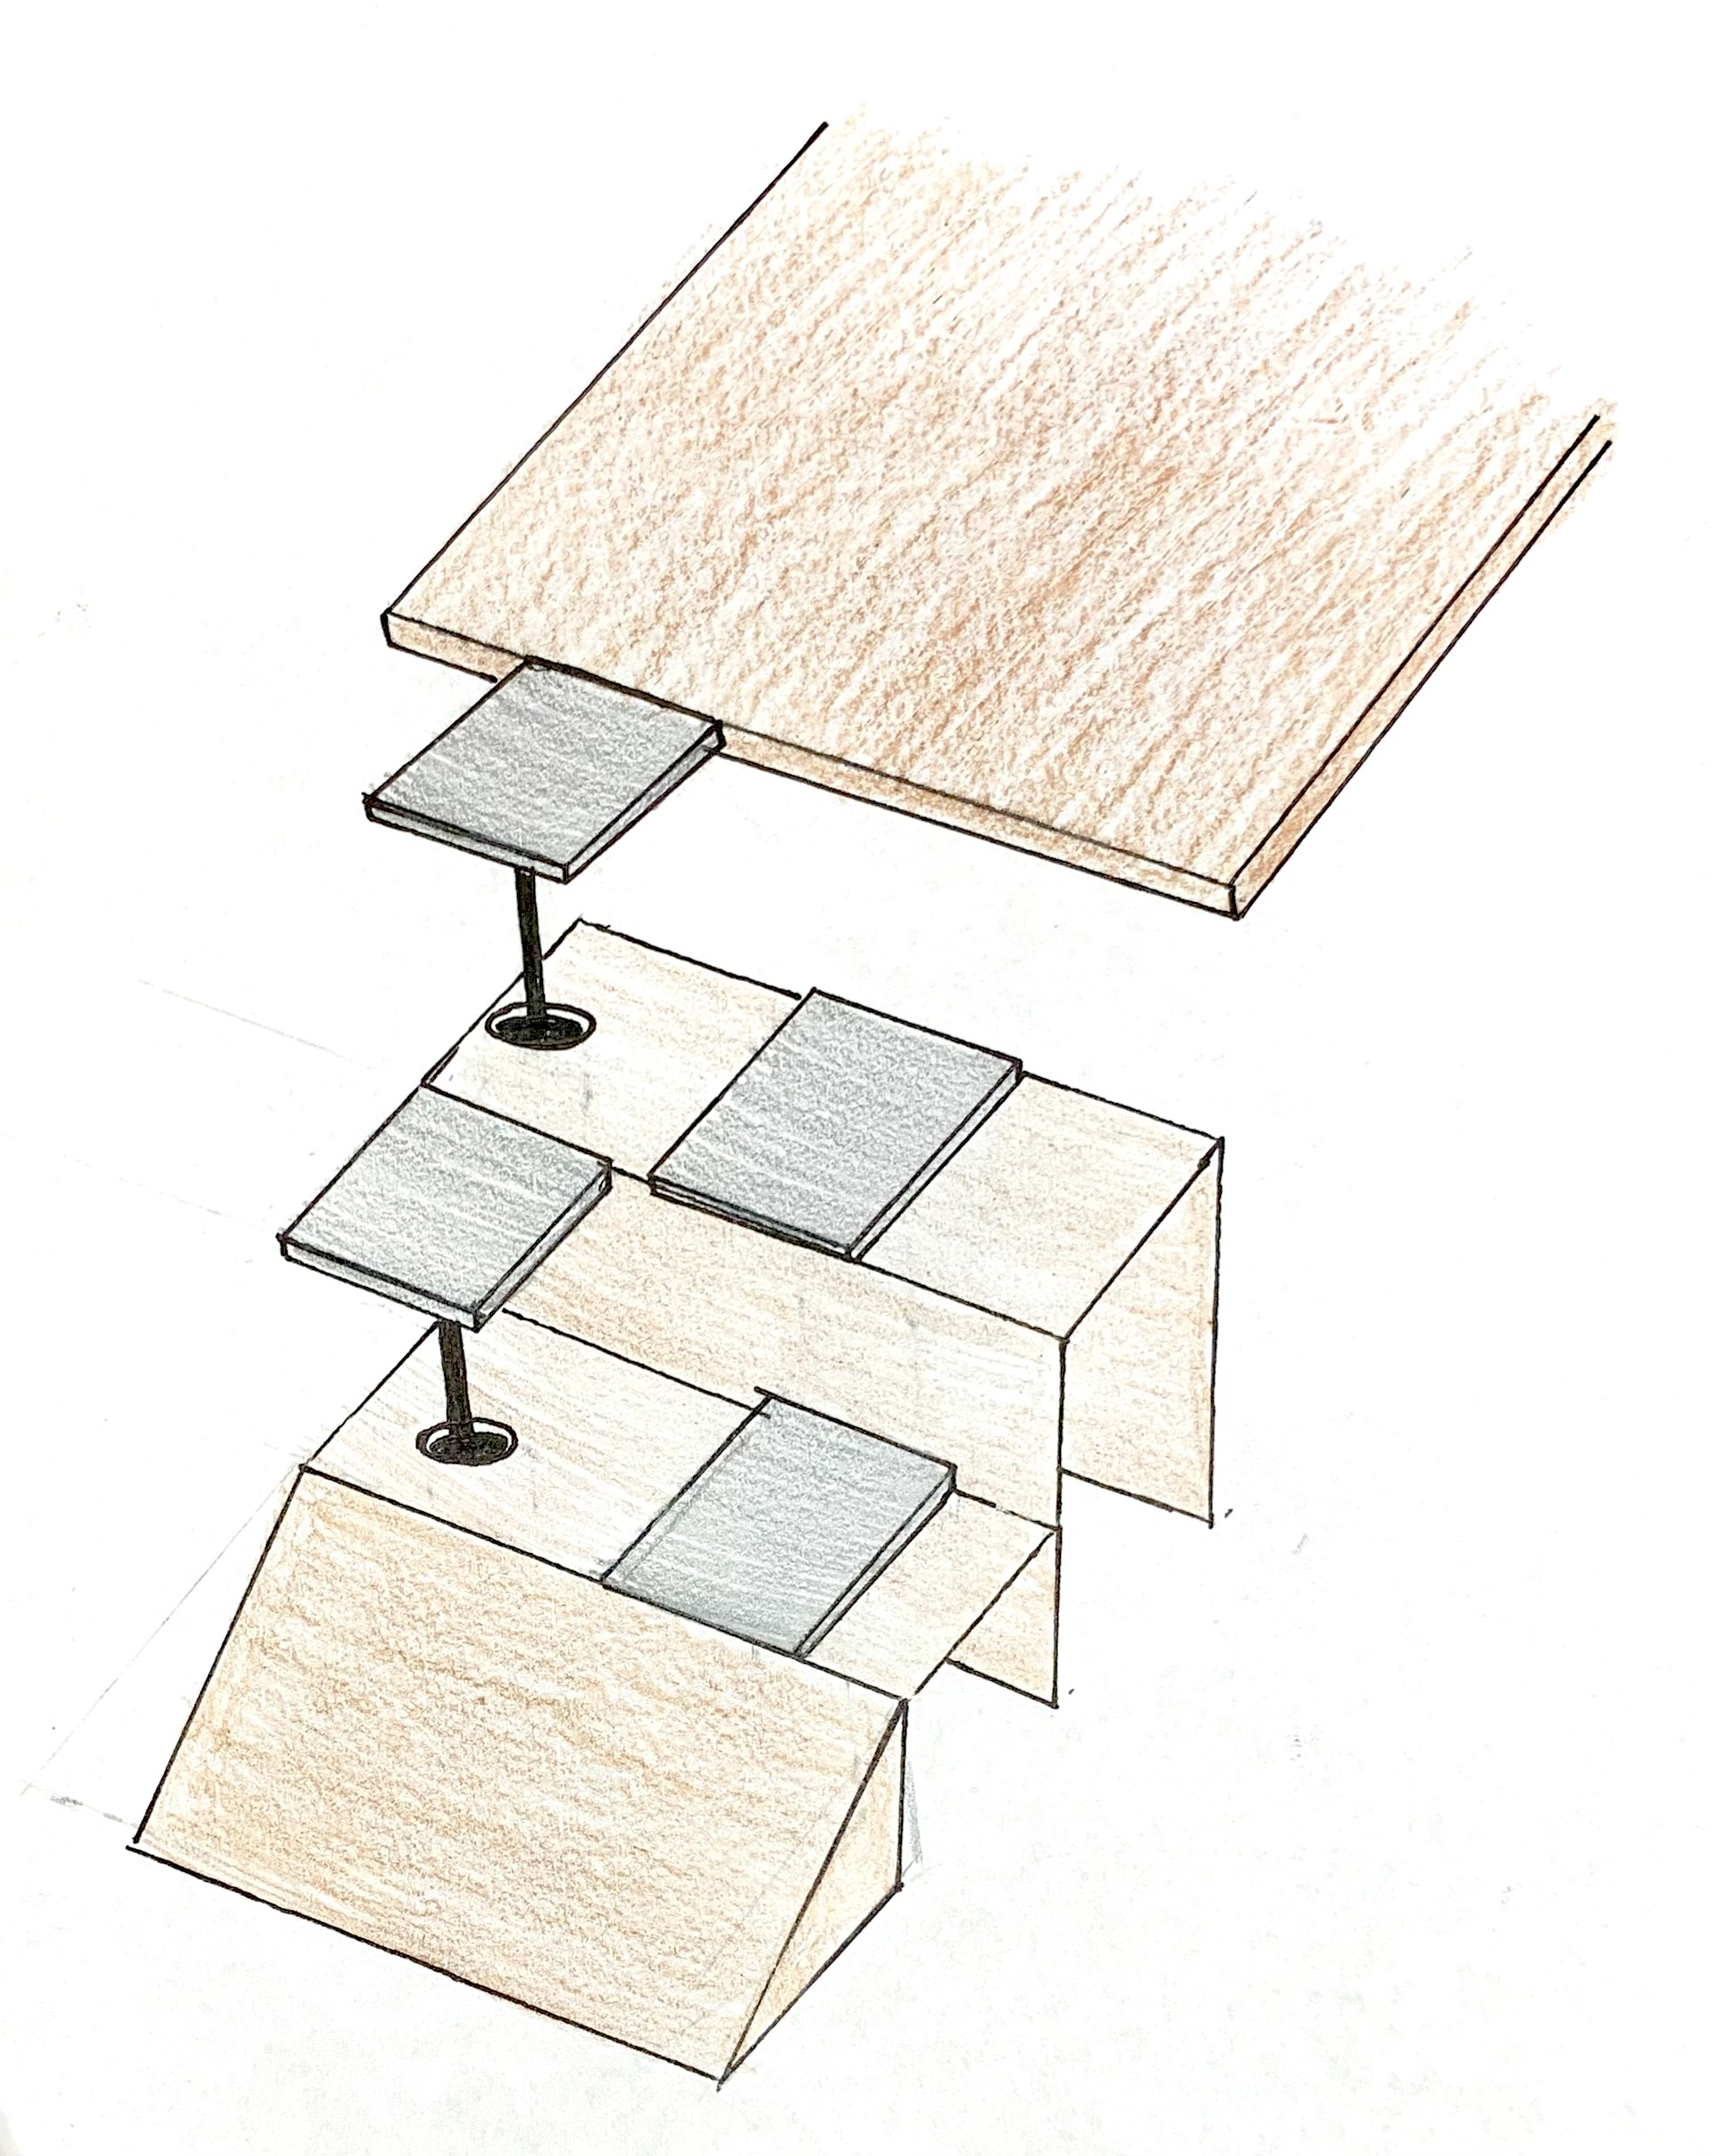
\includegraphics[width=7cm]{IMG_8470.jpg}
\end{subfigure}
\caption{Elevator Concept 1}
This concept utilizes syringes to bring cars down from one level to another. The syringes would be half full of water to add friction and slow cars down so they are not in free fall.
\label{fig:Fig1}
\end{figure}

\begin{figure}[h!]\centering
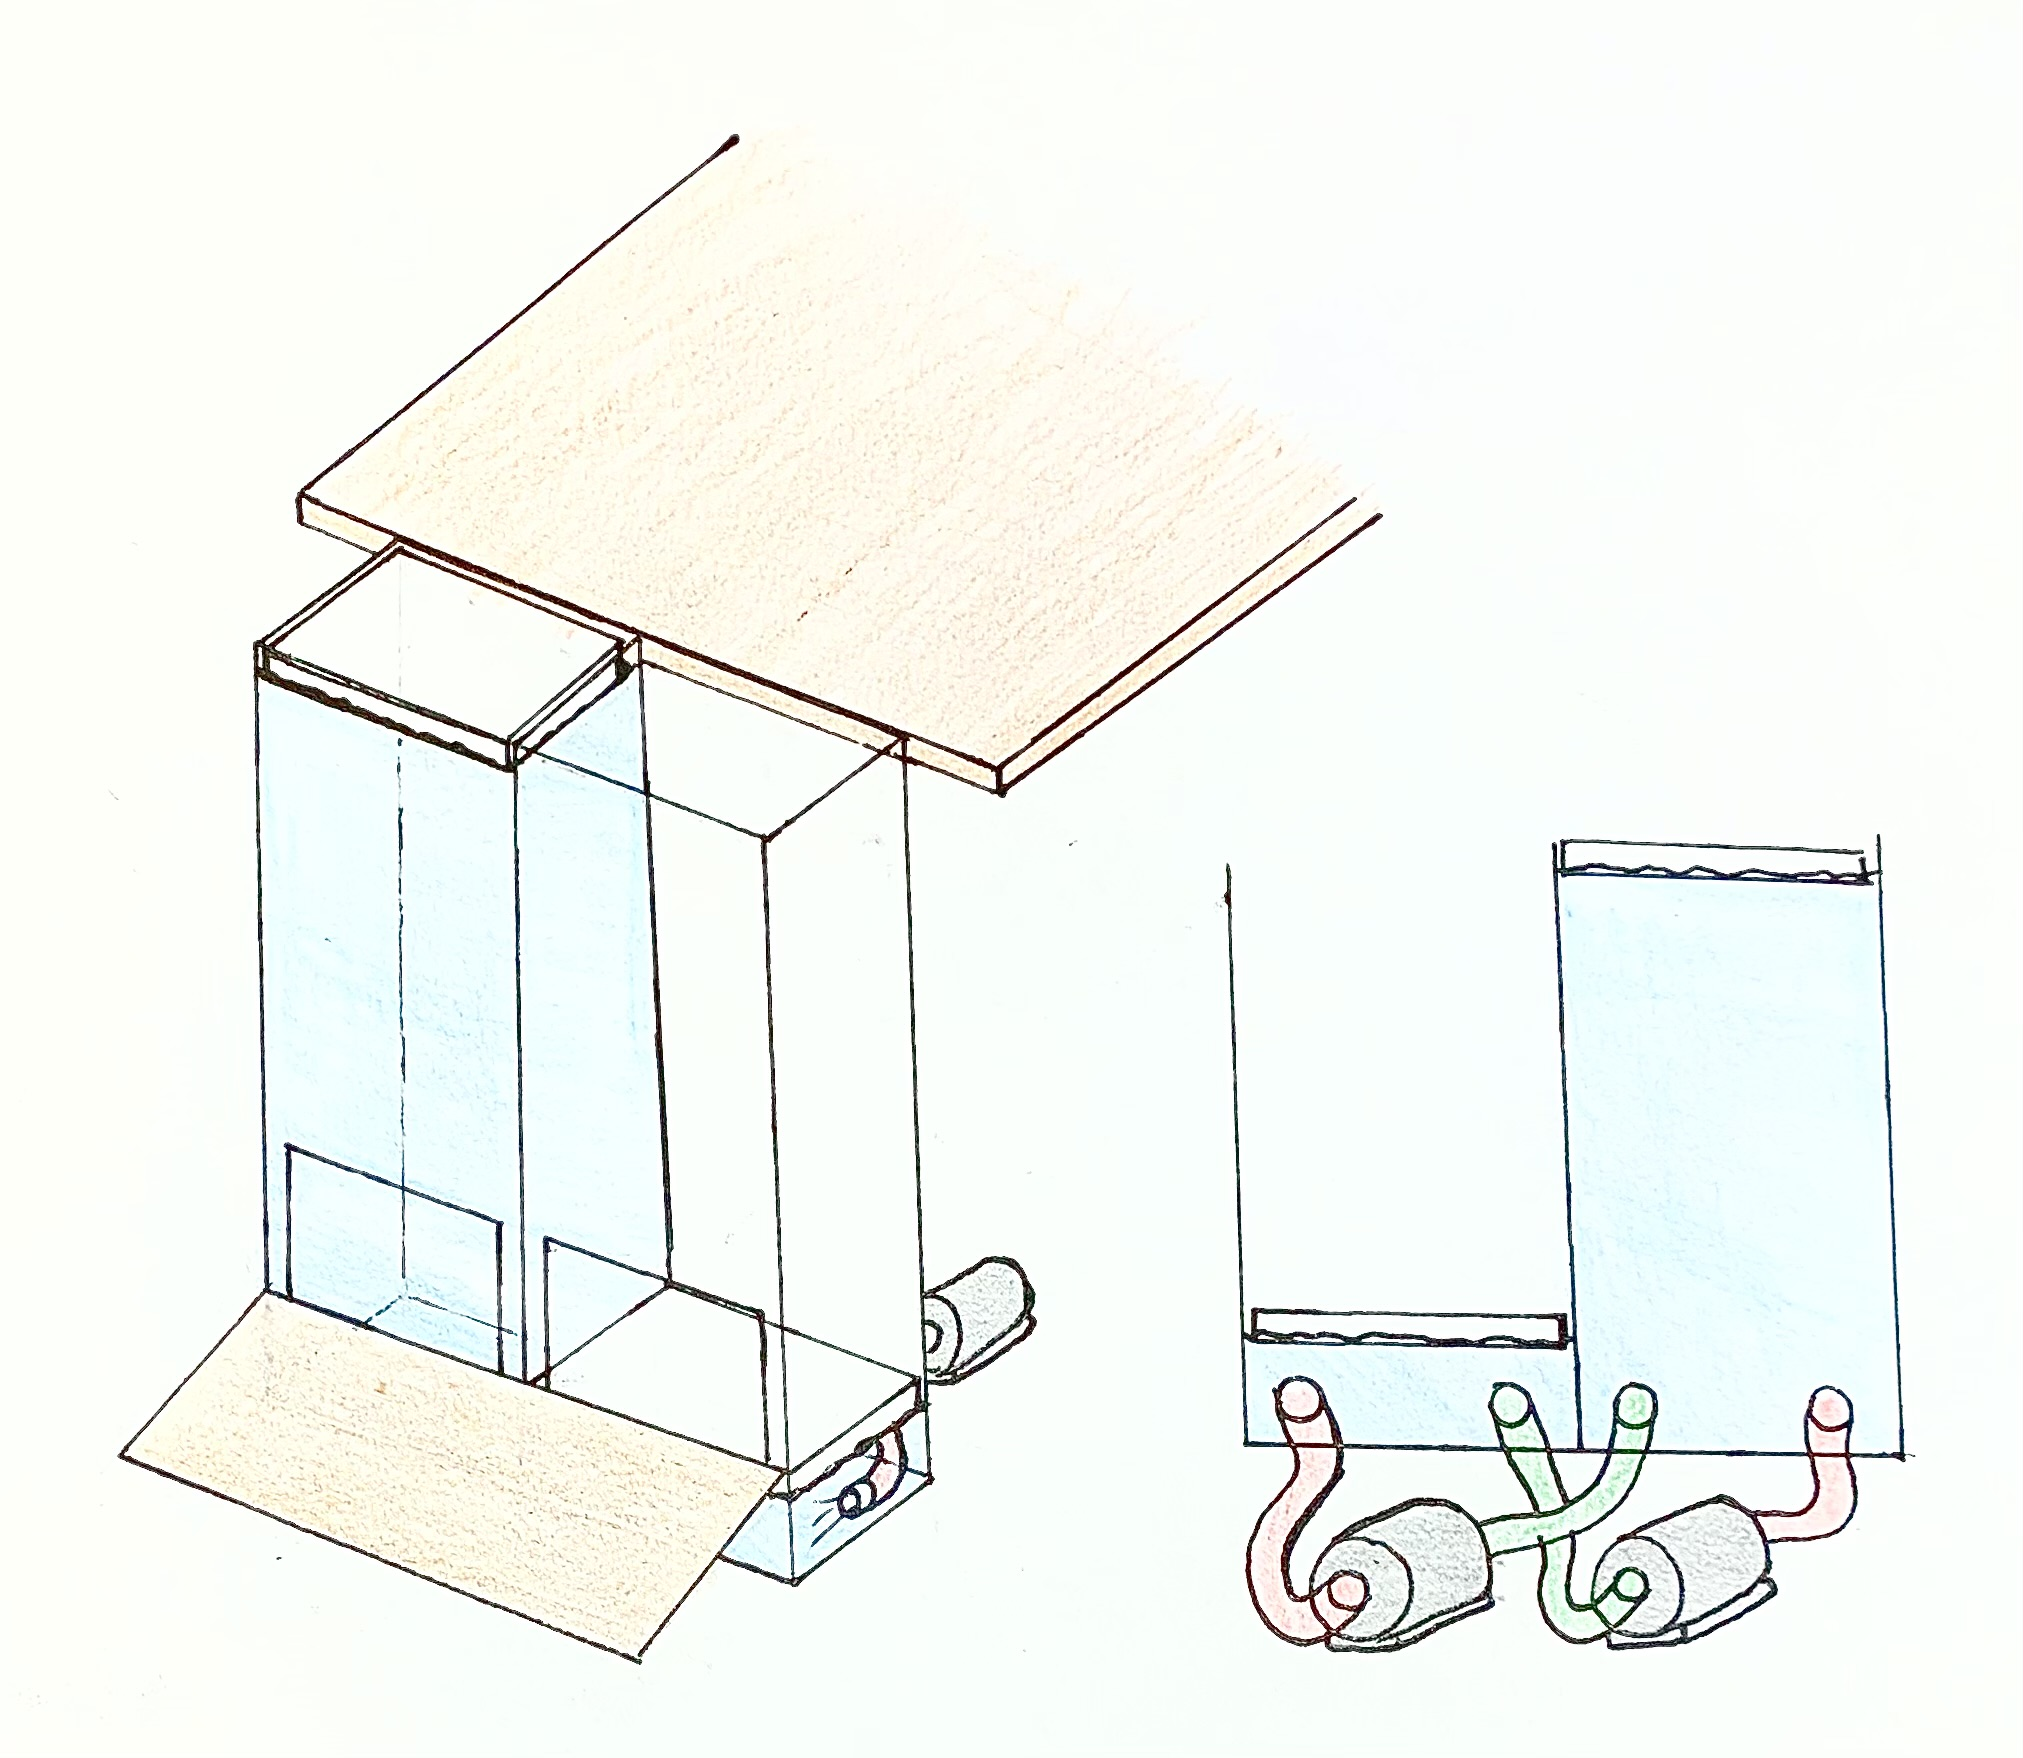
\includegraphics[width=10cm]{IMG_8474.jpg}
\caption{Elevator Concept 2}
This concept used two chambers where two pumps are used to pump water from one chamber to the other. As one chamber is being emptied cars will be lowered on a floating platform until it gets to the bottom.
\label{fig:Fig1}
\end{figure}

\begin{figure}[h!]\centering
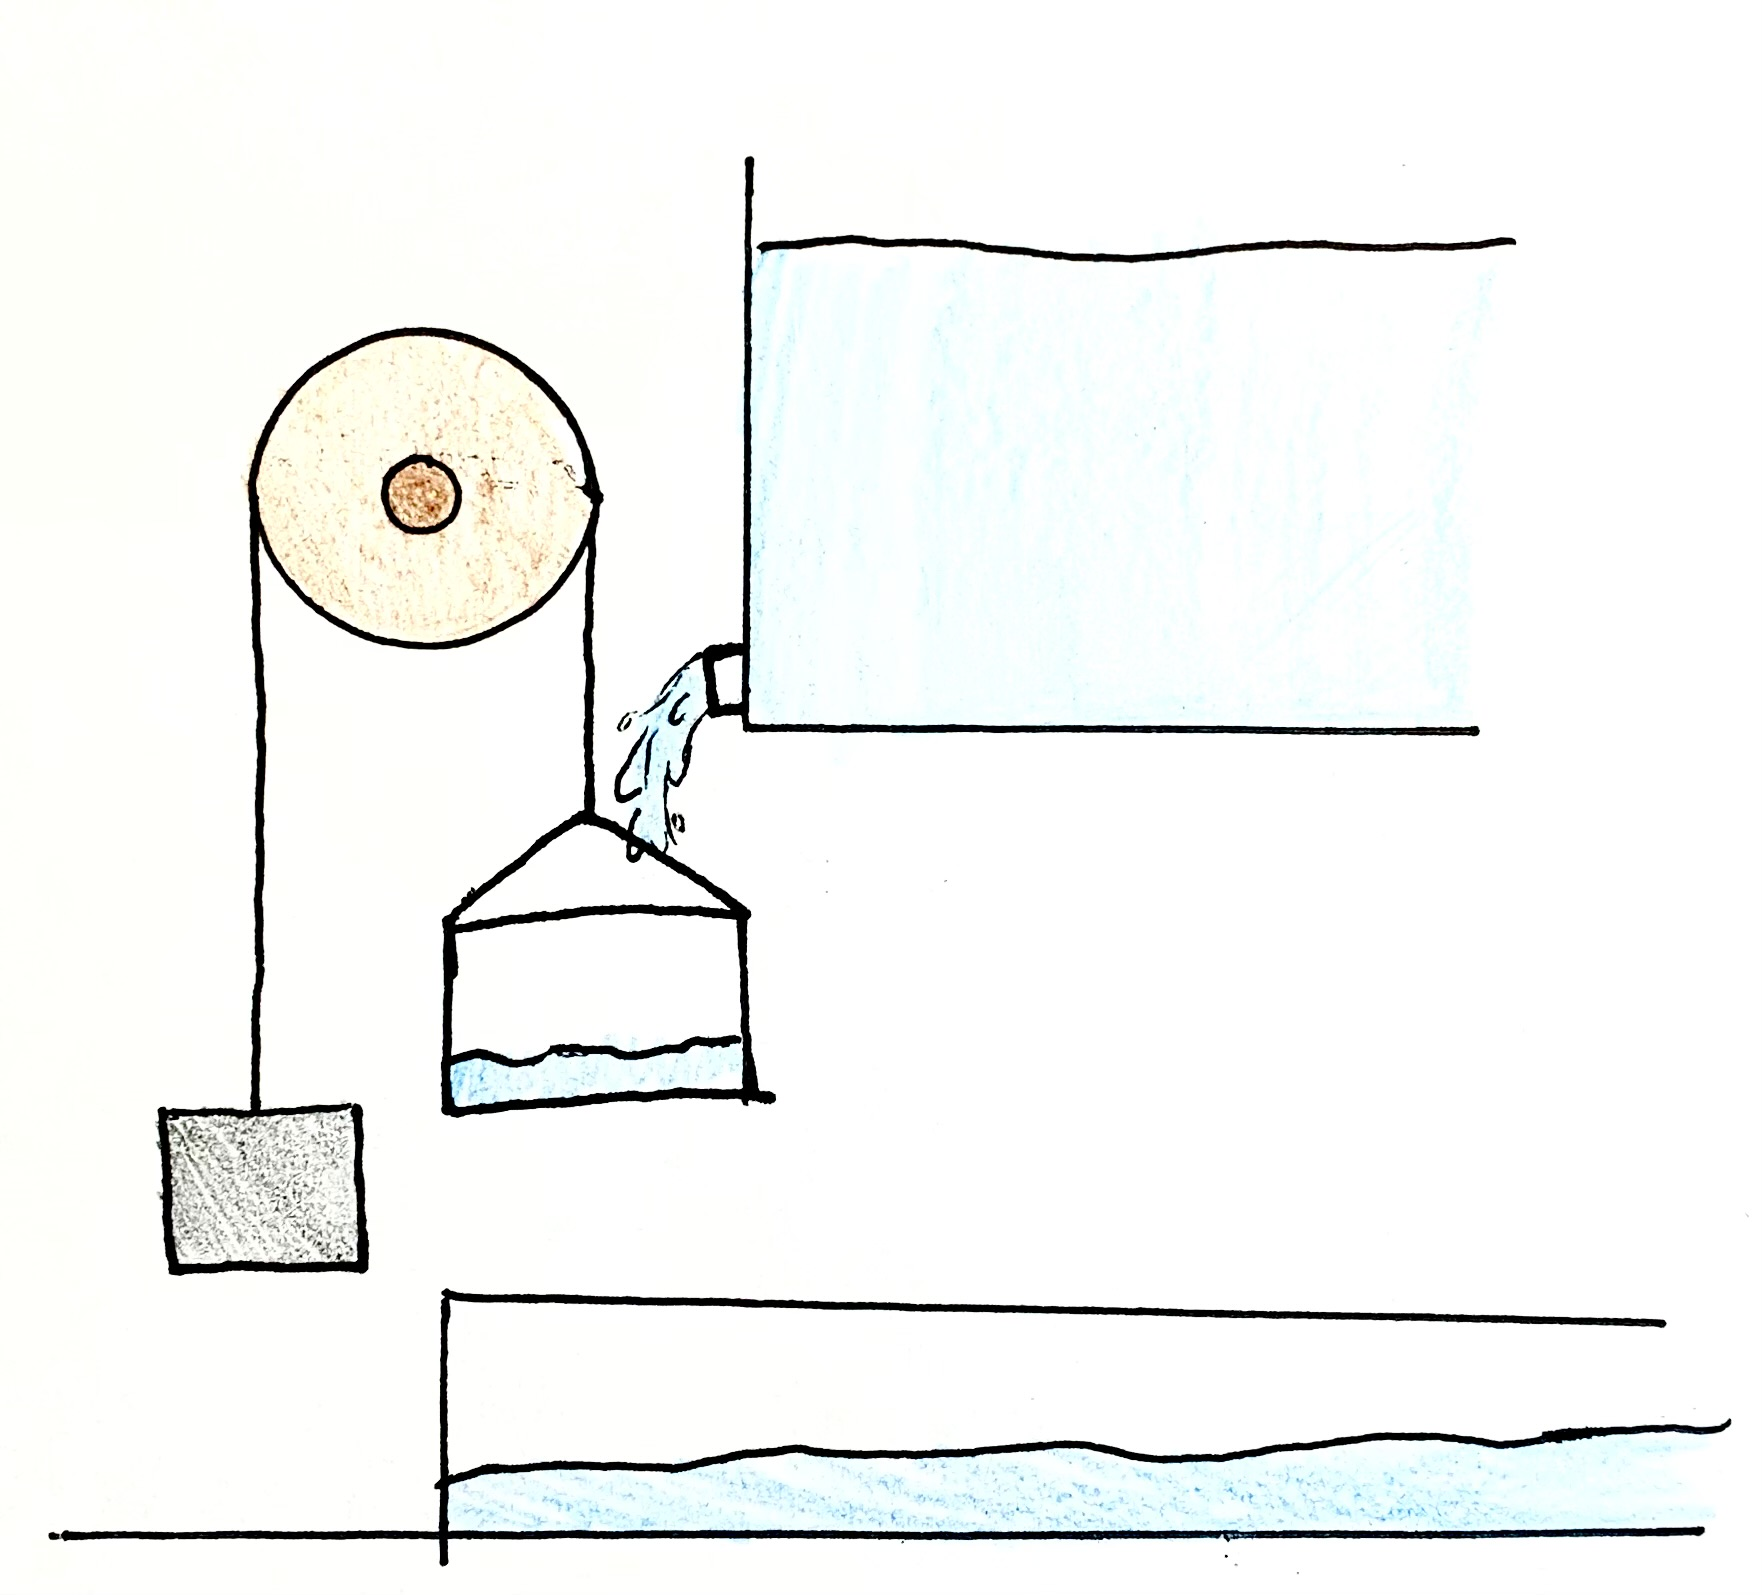
\includegraphics[width=10cm]{IMG_8517.jpg}
\caption{Elevator Concept 3}
This concept incorporated water in container as being a counterweight to bring the cars down. Once the counterweight hits the bottom it would empty allowing the container to go back to the top and refill.
\label{fig:Fig1}
\end{figure}

\subsubsection{Bridge}

\begin{figure}[h!]\centering
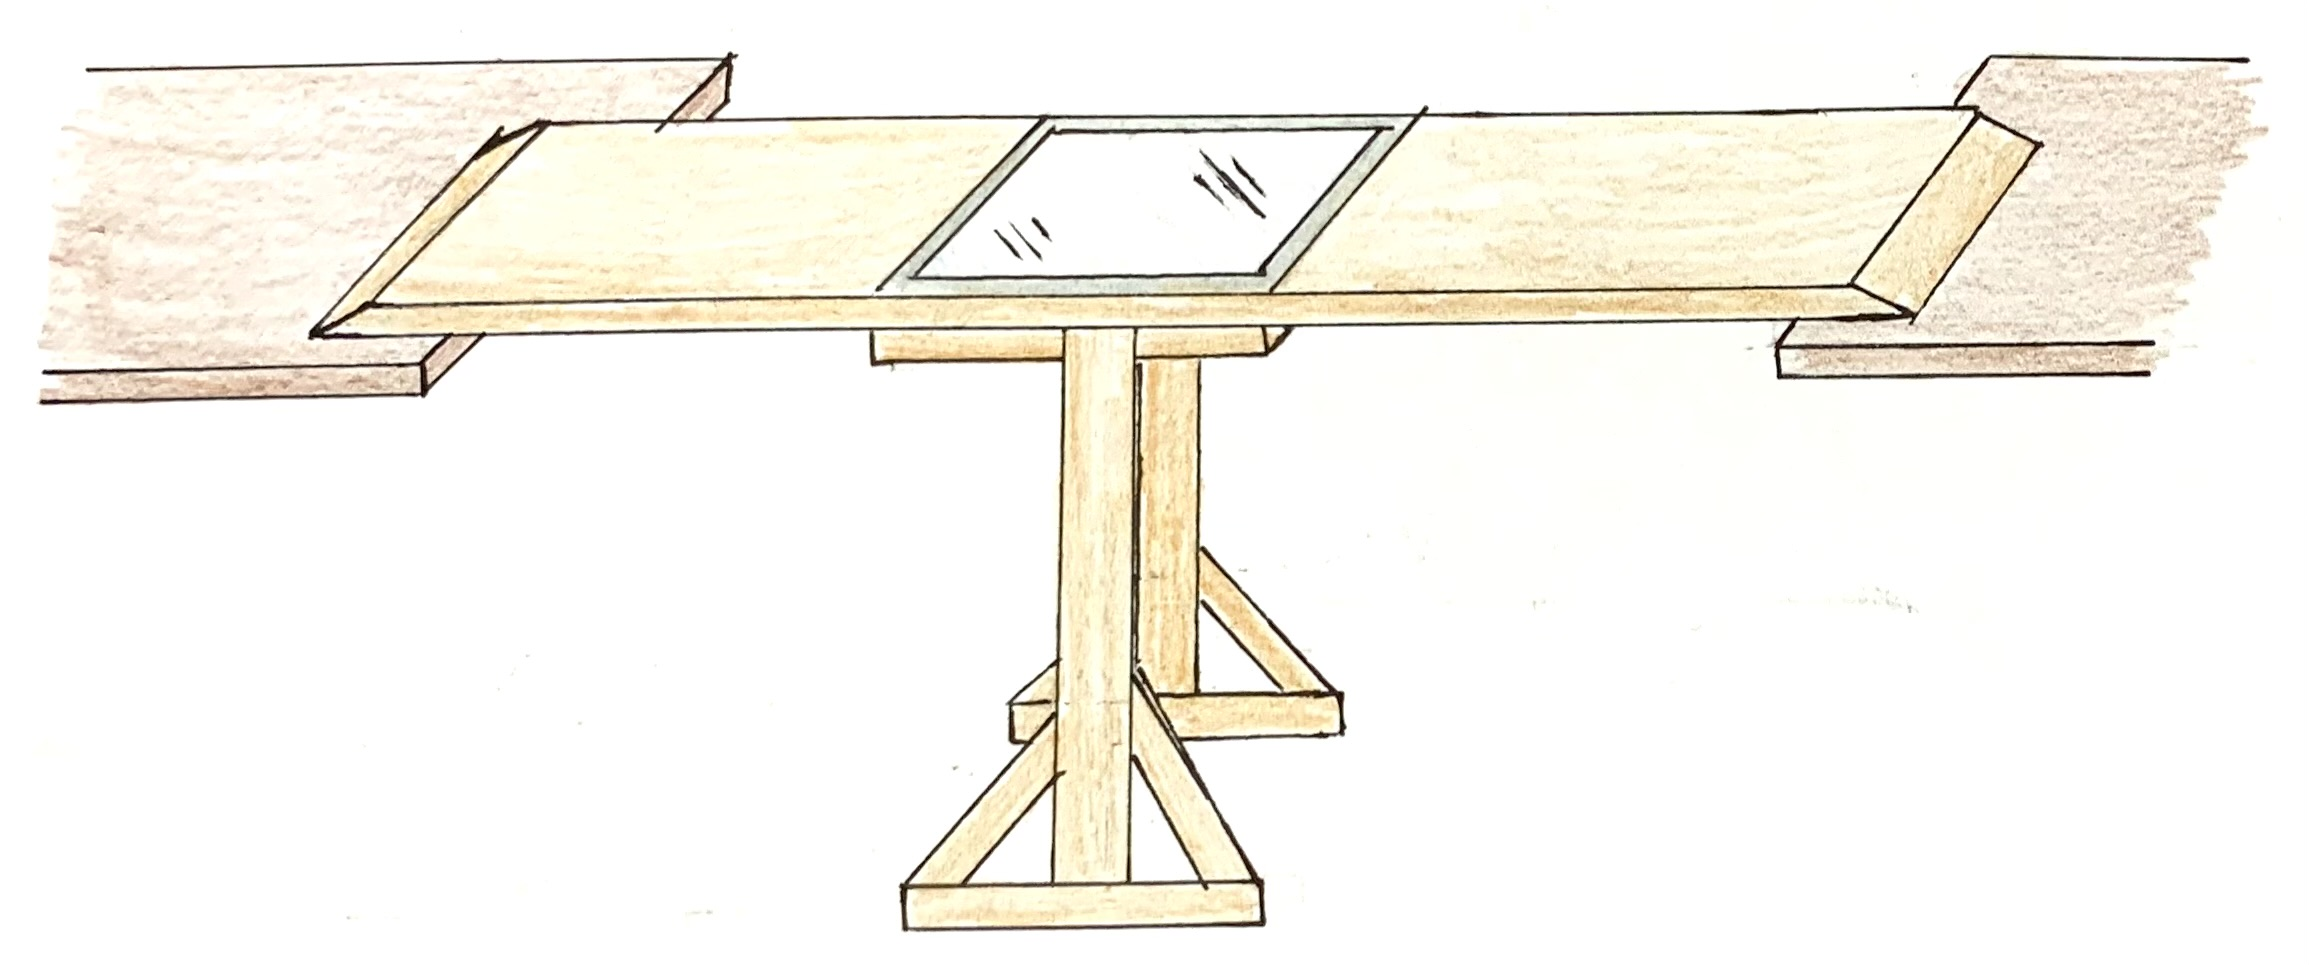
\includegraphics[width=10cm]{Bridge Concept 1.jpg}
\caption{Bridge Concept 1}
This bridge concept is designed with two beams that meet with one low friction zone in the middle. 
\label{fig:Fig1}
\end{figure}

\begin{figure}[h!]\centering
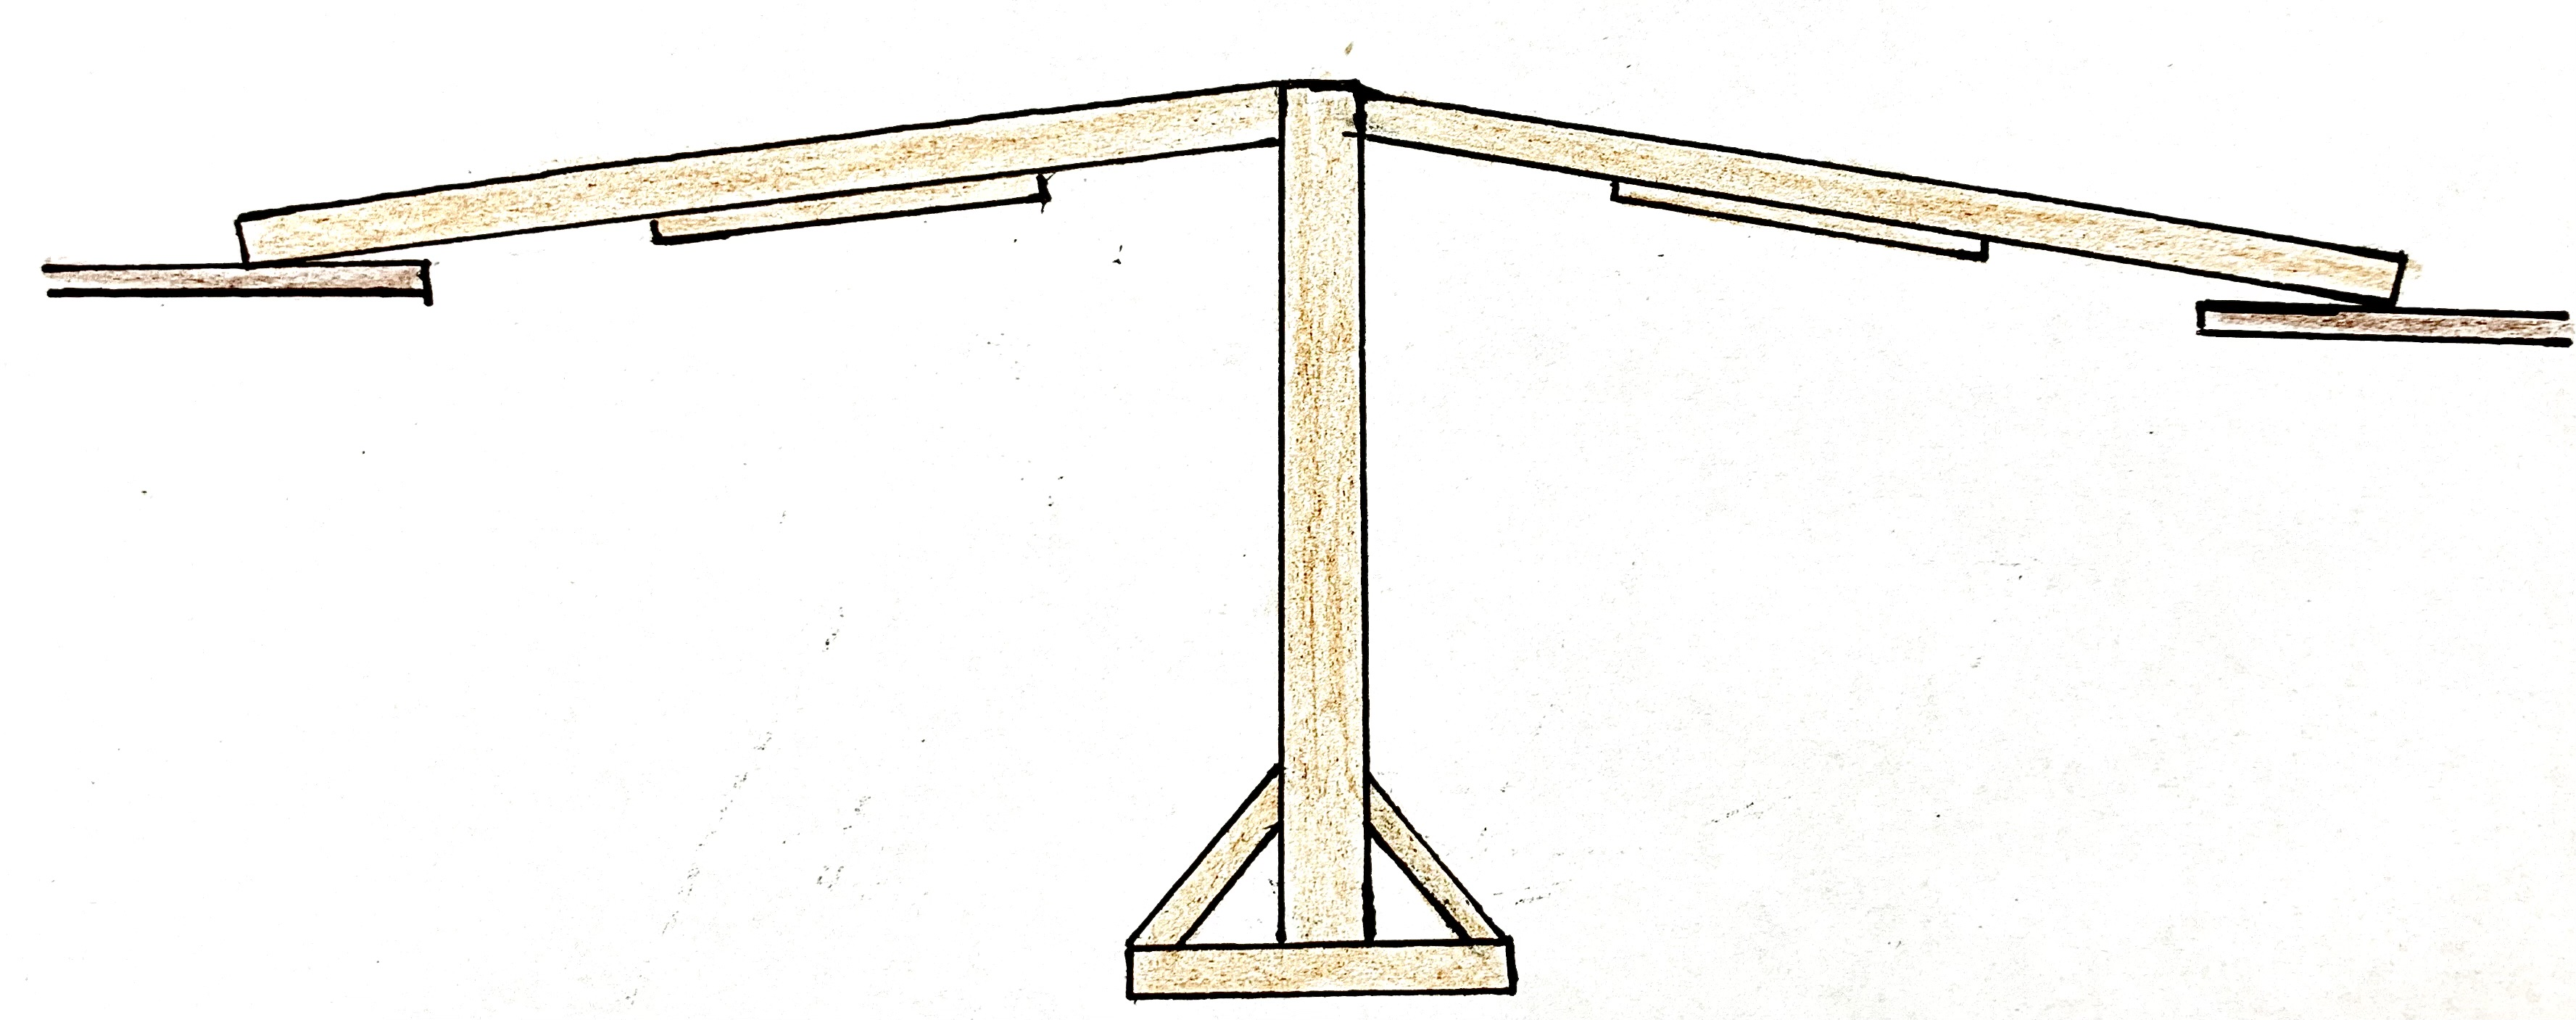
\includegraphics[width=10cm]{Bridge Concept 2.jpg}
\caption{Bridge Concept 2}
This bridge concept has two beams that meet at the highest point in the middle. There are two low friction zones that would be more effective than other concepts because they are at a slant.
\label{fig:Fig1}
\end{figure}

\begin{figure}[h!]\centering
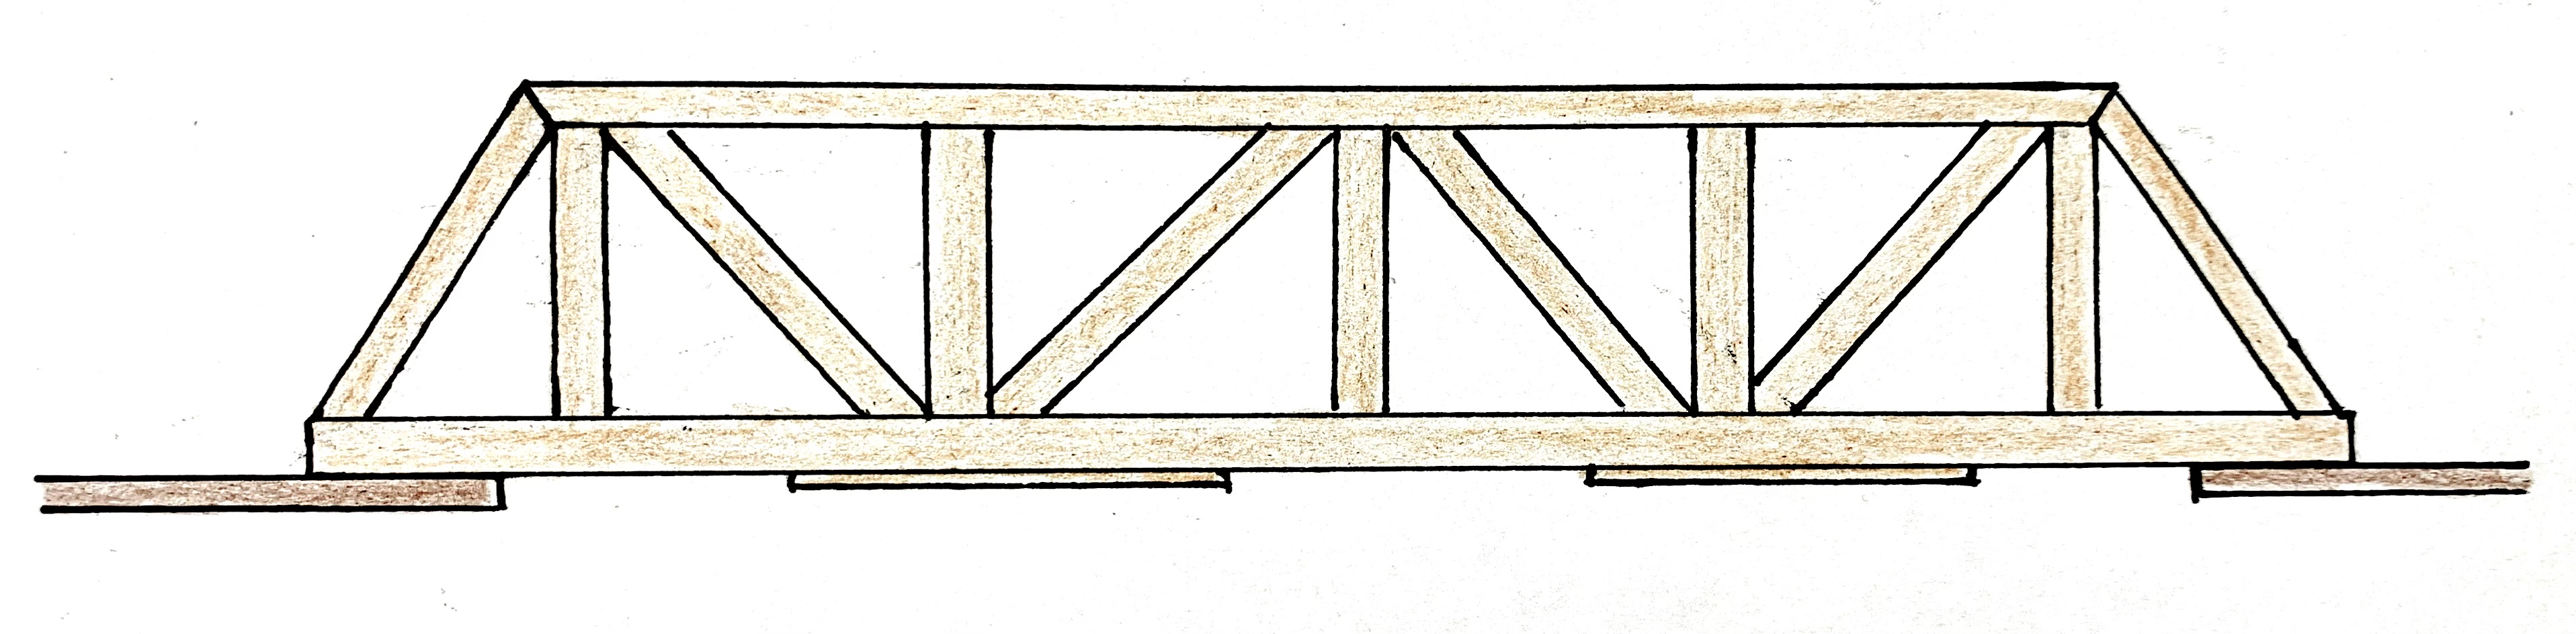
\includegraphics[width=10cm]{Bridge Concept 3.jpg}
\caption{Bridge Concept 3}
This bridge concept is a truss bridge with two low friction zones.
\label{fig:Fig1}
\end{figure}

\subsubsection{Car}

\subsection{Process and Decisions}
\subsubsection{Elevator}
\begin{table}
\begin{center}
\caption{Elevator Decision Matrix}
\begin{tabular}{ | l | c | c | c | c |  }
\hline
\multicolumn{5}{|c|}{\bf{Elevator Decision Matrix}} \\
\hline
\bf{Criteria}& \bf{Weight} &\bf{Concept #1} &\bf{Concept #2} &\bf{Concept #3}\\
\hline
Simplicity & 5 & 9 & 7 & 2 \\
\hline
Cost & 4 & 10 & 1 & 6 \\
\hline
Aesthetic & 3 & 5 & 10 & 7 \\
\hline
Coding/Automation & 1 & 10 & 3 & 5 \\
\hline
Speed & 2 & 5 & 1 & 6 \\
\hline
\multicolumn{2}{|r|}{\bf{Total Score}} & 120 & 74 & 66 \\
\hline
\end{tabular}
\end{center}
\label{table:Table3}
\end{table}

\subsubsection{Bridge}

\begin{table}
\begin{center}
\caption{Bridge Decision Matrix}
\begin{tabular}{ | l | c | c | c | c |  }
\hline
\multicolumn{5}{|c|}{\bf{Bridge Decision Matrix}} \\
\hline
\bf{Criteria}& \bf{Weight} &\bf{Concept #1} &\bf{Concept #2} &\bf{Concept #3}\\
\hline
Cost & 5 & 9 & 8 & 3 \\
\hline
Effectiveness of Ice & 4 & 2 & 9 & 5 \\
\hline
Complexity & 3 & 8 & 7 & 3 \\
\hline
Aesthetic & 2 & 3 & 5 & 8 \\
\hline
Deflection & 1 & 8 & 8 & 2 \\
\hline
\multicolumn{2}{|r|}{\bf{Total Score}} & 97 & 113 & 60 \\
\hline
\end{tabular}
\end{center}
\label{table:Table3}
\end{table}

Cost was ranked the highest because we felt the bridge would be a good spot to try to save money on. Our client wanted us to incorporate ice into our structure so we felt we should weigh in the effectiveness of the ice on how hard it is for a car to cross to make sure the ice is actually doing something. We felt complexity to be important because it is important for our time not to be completely put into the bridge. We found aesthetic to be slightly less important because we were more focused on getting a working bridge. Finally after we found the deflections of each bridge and knew that none of them would collapse, so we decided to rank that with the least weight.

\subsubsection{Car}

%%%%%%%%%%%%%%%%%%%%%%%%%%%%%%%%%%%%%%%%%%%%%%%%%%%%%%%%%%%%%%%%%%%%%%%%%%%%%%%%%%%%%%%%%%%%%%%%%%%%%%%%%%%%%%
\newpage
\section{Detailed Design}
\subsection{Elevator}
\subsubsection{Assumptions}
\subsubsection{Functions and Meeting Specifications}
\subsubsection{Prototypes}
\subsubsection{Manufacturing}
\subsubsection{Final Design}

\subsection{Bridge}
\subsubsection{Assumptions}
\subsubsection{Functions and Meeting Specifications}
\subsubsection{Prototypes}
\subsubsection{Manufacturing}
\subsubsection{Final Design}

\subsection{Car}
\subsubsection{Assumptions}
\subsubsection{Functions and Meeting Specifications}
\subsubsection{Prototypes}
\subsubsection{Manufacturing}
\subsubsection{Final Design}

\newpage
\section{Work Breakdown Structure}
\subsection{Elevator}
\begin{figure}[h!]\centering
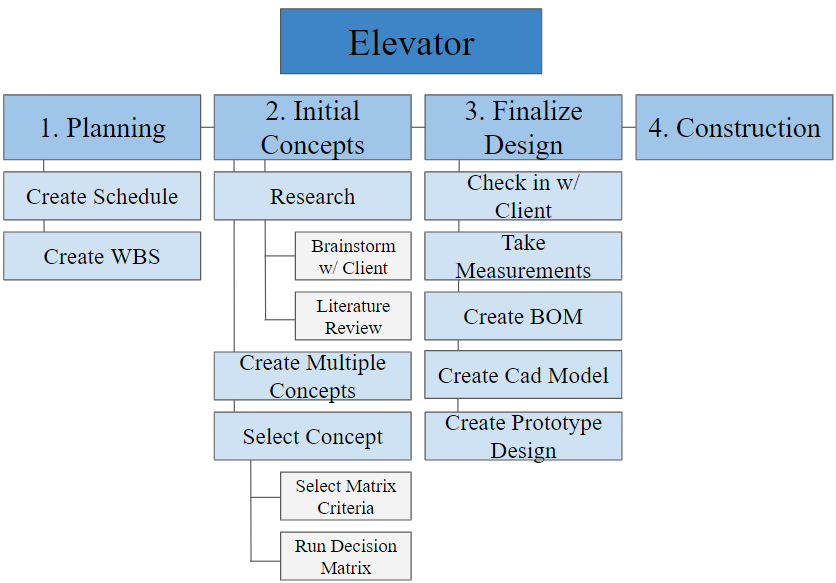
\includegraphics[width=13cm]{Elevator WBS.png}
\end{figure}

\subsection{Ramp}
\begin{figure}[h!]\centering
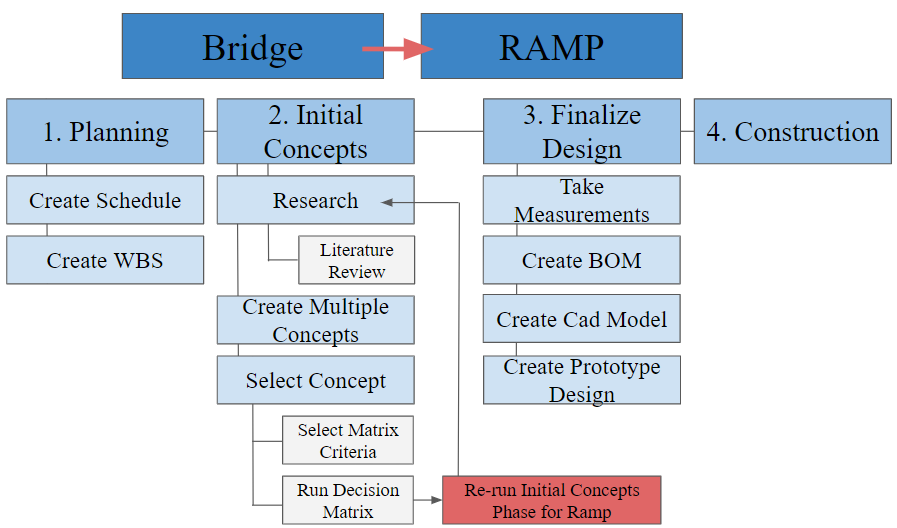
\includegraphics[width=13cm]{Ramp WBS.png}
\end{figure}

\subsection{Car}
\section{Scheduling}
\subsection{First Semester}
\noindent\textbf{Nov 2:} Create Schedule and divide work.

\noindent\textbf{Nov 7:} Create WBS for Car, Elevator, and Bridge. 

\noindent\textbf{Nov 9:} Begin literature review for Car, Elevator, and Bridge. 

\noindent\textbf{Nov 14:} Continue literature review on Elevators & Hydraulics. 

\noindent\textbf{Nov 16:} Meet with client to brainstorm elevator concepts. 

\noindent\textbf{Nov 21:} Finalize Concepts, choose decision matrix criteria, and run decision matrix to select elevator concept. Begin looking at elevator materials.

\noindent\textbf{Nov 23:} Perform bridge literature review and generate bridge concepts. Update report over Thanksgiving break. 

\noindent\textbf{Nov 28:} Finalize bridge concepts and run decision matrix to select final concept. Gather measurements for bridge & elevator. 

\noindent\textbf{Nov 30:} Begin CAD drawings and BOM for elevator. 

\noindent\textbf{Dec 5:} Complete CAD drawings for elevator and BOM for elevator. 

\noindent\textbf{Dec 7:} CAD drawings and BOM for bridge. 

\noindent\textbf{Dec 12:} Complete CAD drawings and BOM for bridge. 

\noindent\textbf{Dec 14:} Make final updates to report. 

\noindent\textbf{Dec 16:} submit working car, prototype design (CAD and control) and Bill of Materials

\subsection{Second Semester}

\section{Bill of Materials}
\subsection{Elevator}
\subsection{Bridge}
\subsection{Car}
\section{Conclusions}


\newpage
\bibliographystyle{IEEEtran}
\bibliography{references}{
[1] M. Fischetti, “New Designs Going Up – Working knowledge on Elevators,” Scientific American, 2009.

[2] “A Guide For Choosing the Type of Elevator You Need,” Pneumatic Vacuum Elevators, 2022.

[3] "Pascal's Law," Clippard. 

}
\newpage
\section*{Appendix}
\addcontentsline{toc}{section}{Appendix}

This is where you'll want to attach your code, computer calculations, hand calculations etc...

You want to include the summarized final results or samples of data within the report itself, but the bulk of your calculations should be here. Anything within the report should be typed, including sample calculations.

Include final (and relevant sample) drawings or figures within the report as it pertains to the text. Only include drawings and/or figures in the appendix if it's supplemental to the text. 
\end{document}
